\chapter{Appendix}

\usetikzlibrary{arrows,shapes,positioning,shadows,trees}

\begin{figure}[!h]
\centering
\tikzset{
every node/.style={draw,text width=2cm,drop shadow},
style1/.style= {rectangle, rounded corners=2pt, thin,align=center,fill=green!30},
style2/.style= {rectangle, rounded corners=6pt, thin,align=center,fill=green!60},
style3/.style= {rectangle,thin,align=left,fill=pink!60}
}



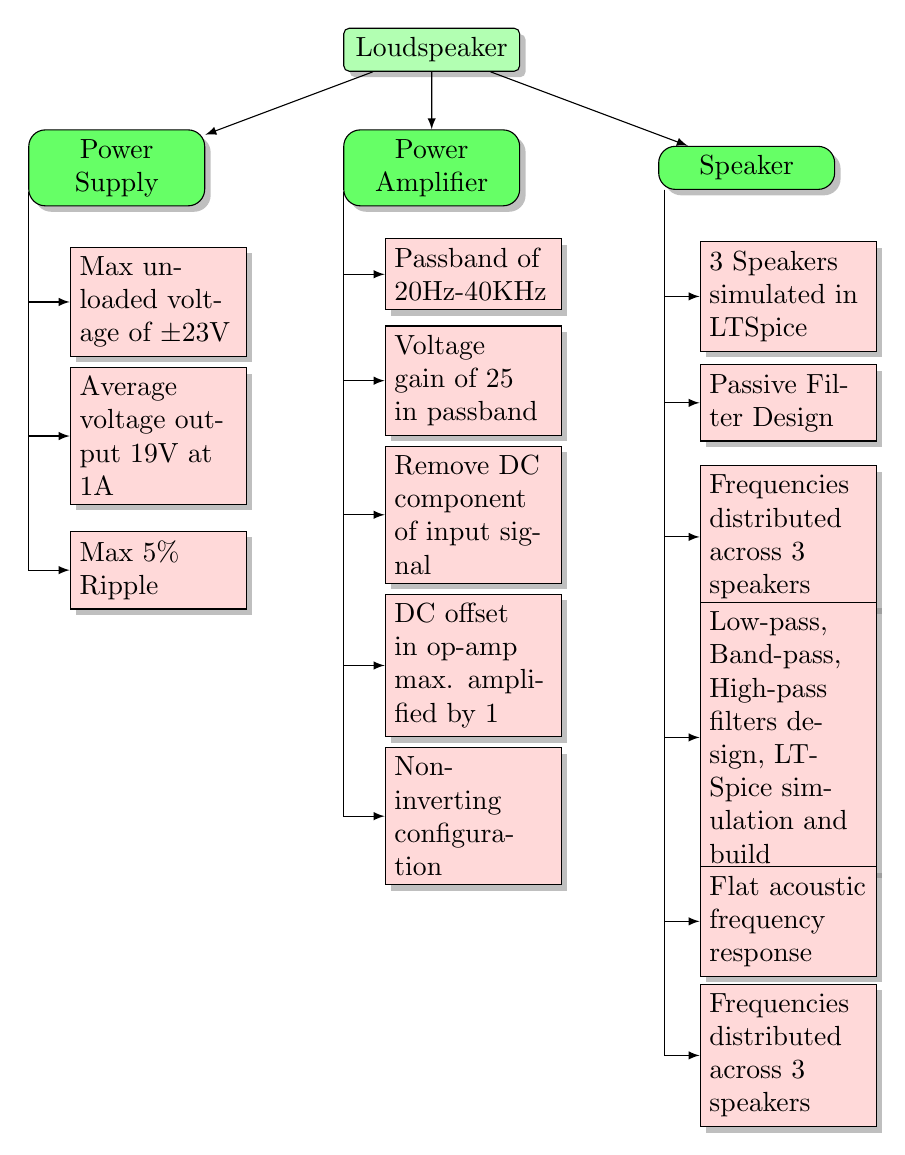
\begin{tikzpicture}[
remember picture,
level 1/.style={sibling distance=40mm},
edge from parent/.style={->,draw},
>=latex]

% the initial tree ("root" and "text nodes")
\node[style1] {Loudspeaker}
child {node[style2] (c1) {Power Supply}}
child {node[style2] (c2) {Power Amplifier}}
child {node[style2] (c3) {Speaker}};

% the nodes below each of the "text" nodes
\node [style3,below of = c1,xshift=15pt,yshift=-20pt] (c11) {Max unloaded voltage of \(\pm\)23V};
\node [style3,below of = c11,yshift=-20pt] (c12) {Average voltage output 19V at 1A};
\node [style3,below of = c12,yshift=-20pt] (c13) {Max 5\% Ripple};

\node [style3,below of = c2,xshift=15pt,yshift=-10pt] (c21) {Passband of 20Hz-40KHz};
\node [style3,below of = c21,yshift=-10pt] (c22) {Voltage gain of 25 in passband};
\node [style3,below of = c22,yshift=-20pt] (c23) {Remove DC component of input signal};
\node [style3,below of = c23,yshift=-26pt] (c24) {DC offset in op-amp max. amplified by 1};
\node [style3,below of = c24,yshift=-26pt] (c25) {Non-inverting configuration};

\node [style3,below of = c3,xshift=15pt,yshift=-18pt] (c31) {3 Speakers simulated in LTSpice};
\node [style3,below of = c31,yshift=-10pt] (c32) {Passive Filter Design};
\node [style3,below of = c32,yshift=-20pt] (c33) {Frequencies distributed across 3 speakers};
\node [style3,below of = c33,yshift=-44pt] (c34) {Low-pass, Band-pass, High-pass filters design, LTSpice simulation and build};
\node [style3,below of = c34,yshift=-38pt] (c35) {Flat acoustic frequency response};
\node [style3,below of = c35,yshift=-20pt] (c36) {Frequencies distributed across 3 speakers};


% lines from each "text" node to every one of its "children"
\foreach \value in {1,2,3}
  \draw[->] (c1.195) |- (c1\value.west);

\foreach \value in {1,...,5}
  \draw[->] (c2.195) |- (c2\value.west);

\foreach \value in {1,...,6}
  \draw[->] (c3.195) |- (c3\value.west);
  

\end{tikzpicture}
    \captionsetup{justification=centering}
    \caption{Work breakdown structure}
    \label{tab:breakdown}
\end{figure}